Als Radius eines Schwarzen Lochs der Masse $M$ nimmt man den Schwarzschildradius $r_\mathrm{S} = 2\,G\,M/c^2$. Die mittlere Dichte ist dann
\begin{align}
 \rho &= \frac{M}{\frac{4}{3}\pi\,r_\mathrm{S}^3}
   = \frac{3\,M}{4\pi}\cdot\frac{c^6}{8\,G^3 M^3}
   = \result{\frac{3\,c^6}{32\pi\,G^3\,M^2}}
\end{align}
Die Dichte ist umgekehrt proportional zum Quadrat der Masse. Für ein Schwarzes Loch von einer Sonnenmasse ($M_\odot = \MSoO$, FoTaBe S.~211) ist
\begin{align}
 \rho_\odot &= \rhSF = \rhS \approx \rhSS{2}
\end{align}
Damit ist $\rho = \rho_\odot\cdot\left(M_\odot/M\right)^2$. Im doppelt logarithmischen Diagramm ist das eine Gerade mit der Steigung $-2$:

\begin{center}
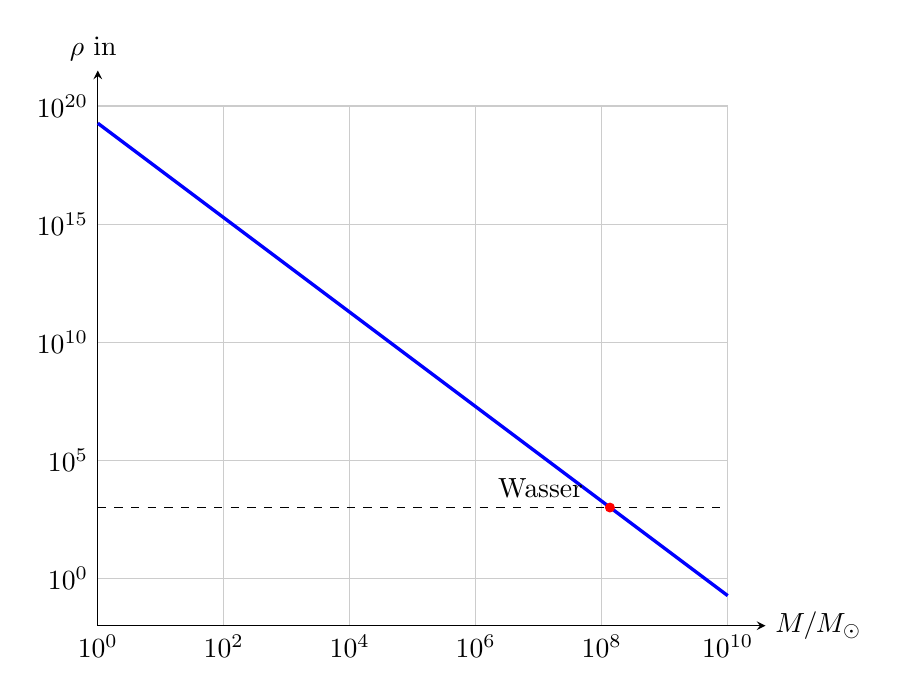
\begin{tikzpicture}[>=stealth, xscale=0.8, yscale=0.3]
 \foreach \x in {0,2,4,6,8,10} {
  \draw[gray!40] (\x,-2) -- (\x,20);
  \node[below] at (\x,-2) {$10^{\x}$};
 }
 \foreach \y in {0,5,10,15,20} {
  \draw[gray!40] (0,\y) -- (10,\y);
  \node[left] at (0,\y) {$10^{\y}$};
 }
 \draw[->] (0,-2) -- (10.6,-2) node[right] {$M/M_\odot$};
 \draw[->] (0,-2) -- (0,21.5) node[above] {$\rho$ in $\si{\kilogram\per\cubic\meter}$};
 \draw[blue, very thick] (0,19.27) -- (10,-0.73);
 \draw[dashed] (0,3) -- (10,3);
 \node[anchor=south west] at (6.2,3) {Wasser};
 \fill[red] (8.13,3) circle (0.08 and 0.21);
\end{tikzpicture}
\end{center}

Leichte Schwarze Löcher sind ungeheuer dicht, sehr massereiche dagegen nicht: Ein Schwarzes Loch hat die mittlere Dichte von Wasser ($\rho_\mathrm{W} = \rhWO$), wenn
\begin{align}
 M &= \MWaF = \MWa \approx \nWaS{2}\,M_\odot
\end{align}
(roter Punkt im Diagramm).
